\documentclass[10pt,a4paper]{article}

\usepackage{appendix}
\usepackage{graphicx}
\usepackage{parskip}
\usepackage{listings}
\usepackage{caption}
\usepackage{subcaption}
\usepackage{amsmath}
\usepackage{listings}
\usepackage{xcolor}
\usepackage[most]{tcolorbox}

%%%%%%%%%%%%%%%%%%%%%%%%%%%%%%%%%%%%%%%%%%%%%%%%%%%%%%%%%%%%%%%%%%%%%%%%%%%%%%%%%%%%%%%%%%%%%%%%%%%%%%%%%%
\definecolor{codegreen}{rgb}{0,0.6,0}
\definecolor{codegray}{rgb}{0.5,0.5,0.5}
\definecolor{codepurple}{rgb}{0.58,0,0.82}
\definecolor{backcolour}{rgb}{1,1,1}

\lstdefinestyle{mystyle}
{
    backgroundcolor=\color{backcolour},   
    commentstyle=\color{codegreen},
    keywordstyle=\color{magenta},
    numberstyle=\tiny\color{codegray},
    stringstyle=\color{codepurple},
    basicstyle=\ttfamily\footnotesize,
    breakatwhitespace=false,         
    breaklines=true,                 
    captionpos=b,                    
    keepspaces=true,                 
    numbers=left,                    
    numbersep=5pt,                  
    showspaces=false,                
    showstringspaces=false,
    showtabs=false,                  
    tabsize=2
}

\lstset{style=mystyle}
%%%%%%%%%%%%%%%%%%%%%%%%%%%%%%%%%%%%%%%%%%%%%%%%%%%%%%%%%%%%%%%%%%%%%%%%%%%%%%%%%%%%%%%%%%%%%%%%%%%%%%%%%%

\lstset{basicstyle=\ttfamily, breaklines = true, tabsize=2}
\graphicspath{ {./Images/} }
\setlength{\parskip}{1em}
\begin{document}


%%%%%%%%%%%%%%%%%%%%%%%%%%%%%%%%%%%%%%%%%%%%%%%%%%%%%%%%%%%%%%%%%%%%%%%%%%%%%%%%%%%%%%%%%%%%%%%%%%%%%%%%%%

\begin{titlepage}
	\centering
	{\scshape\LARGE Imperial College London \par}
	\vspace{1cm}
    {\scshape\Large Mathematics: Year 2\par}
    \vspace{1.5cm}
	{\huge\bfseries Linear Algebra \par}
	\vspace{2cm}
	{\Large\ Xin Wang }
	\vfill
	{\large \today\par}
\end{titlepage}

%%%%%%%%%%%%%%%%%%%%%%%%%%%%%%%%%%%%%%%%%%%%%%%%%%%%%%%%%%%%%%%%%%%%%%%%%%%%%%%%%%%%%%%%%%%%%%%%%%%%%%%%%%

\begin{abstract}
    As mentioned in the previous chapter, if no solution is present i.e. the system is inconsistent,
    then it has to be dealt with another way. No exact solutions can be found, it has to be approximated.
\end{abstract}

%%%%%%%%%%%%%%%%%%%%%%%%%%%%%%%%%%%%%%%%%%%%%%%%%%%%%%%%%%%%%%%%%%%%%%%%%%%%%%%%%%%%%%%%%%%%%%%%%%%%%%%%%%

\tableofcontents
\pagebreak

%%%%%%%%%%%%%%%%%%%%%%%%%%%%%%%%%%%%%%%%%%%%%%%%%%%%%%%%%%%%%%%%%%%%%%%%%%%%%%%%%%%%%%%%%%%%%%%%%%%%%%%%%%
\section{Orthogonality}

This concept is moved to orthogonal subspaces and orthogonal bases and orthogonal matrices. Recall
that the two vectors are orthogonal when their dot product is zero:  $v . w = v^T w  =  0$. Since it
is perpendicular, Pythagoras can be used:
\begin{align*}
    ||v||^2 + ||w||^2 = ||v+w||^2
\end{align*}

Recall the four fundamental subspaces that reveal what a matrix really does. A matrix multiplies a
vector:  $A$ times $x$.  
\begin{itemize}
    \item At the first level this is only numbers.
    \item At the second level $Ax$ is a combination of column vectors.
    \item At third level is with subspaces. 
\end{itemize}   
\begin{figure} [h!]
    \centering
    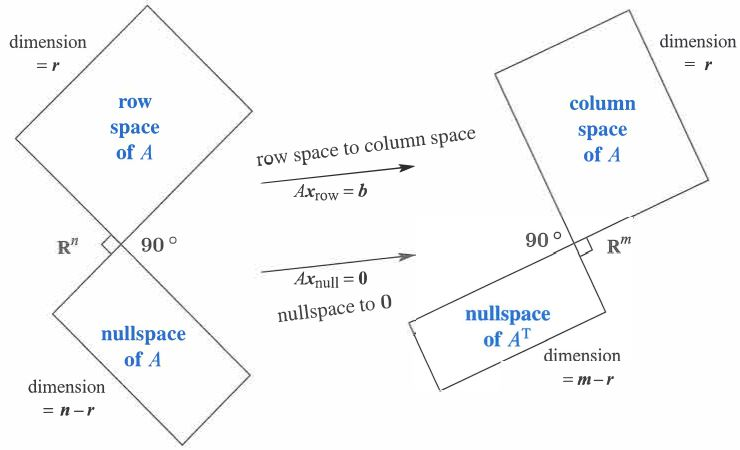
\includegraphics[scale=0.7]{sub.JPG}
\end{figure}

With the concept of orthogonality:
\begin{itemize}
    \item \textbf{The row space is perpendicular to the nullspace}.  
    
    Every row of $A$ is perpendicular to every solution of $Ax = 0$. That gives the $90$ degree
    angle on the left side of the figure. This perpendicularity of subspaces is what is of interest.

    \item \textbf{The column space is perpendicular to the nullspace of $A^T$}.
    
    When $b$ is outside the column space, solving $Ax = b$ is impossible. This nullspace of 
    $A^T$ comes into its own. It will contain the error $e  =  b - Ax$ in the "least-squares" solution. 
    Least squares is the key application of linear algebra in this chapter. 
\end{itemize}

\begin{tcolorbox}[breakable,colback=white]
    \textbf{Orthogonal subspaces}: $v^T w = 0$ for all $v$ in $V$ and all $w$ in $W$.
\end{tcolorbox}

Note: Orthogonality is impossible when $dim (V) + dim (W)  >  dim (whole space)$.  Two planes (dimensions 2 and 2 in $R^3$) cannot be orthogonal subspaces.

The crucial examples for  linear algebra come fr om the  four fundamental subspaces. Zero is the
only point where the nullspace meets the row space. 

\begin{tcolorbox}[breakable,colback=white]
    Every vector $x$ in the nullspace is perpendicular to every row of $A$, because $Ax  =  0$. 
    The null space $N(A)$ and the row space $C(A^T)$ are orthogonal subspaces of $R^n$.
\end{tcolorbox}
\begin{figure} [h!]
    \centering
    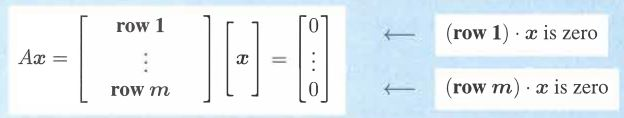
\includegraphics[scale=0.7]{oth.JPG}
\end{figure}

%%%%%%%%%%%%%%%%%%%%%%%%%%%%%%%%%%%%%%%%%%%%%%%%%%%%%%%%%%%%%%%%%%%%%%%%%%%%%%%%%%%%%%%%%%%%%%%%%%%%%%%%%%
\subsection{Orthogonal complements}

The fundamental subspaces are more than just orthogonal (in  pairs). Their dimensions are also
just right. 

Consider two lines that are perpendicular in $R^3$. Those lines \textbf{could not be} the row
space and nullspace of a $3 \times 3$ matrix. The lines have dimensions 1 and 1, adding to 2.
But the correct dimensions $n - r$ must add to $n= 3$. 

The fundamental subspaces of a 3 by 3 matrix have dimensions 2 and 1, or 3 and 0. Those pairs of
subspaces are not only orthogonal, they are orthogonal complements.

\begin{tcolorbox}[breakable,colback=white]
\textbf{Orthogonal complement} (of a subspace $V$): Denoted $V^{\perp}$, contains every vector that is 
perpendicular to $V$.
\end{tcolorbox}
\begin{figure} [h!]
    \centering
    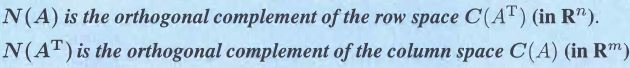
\includegraphics[scale=0.7]{com.JPG}
\end{figure}

The two subspaces are orthogonal complements if:
\begin{align*}
    \text{dim}N(A)+ \text{dim}C(A T ) = \text{dim} R^n = n \; \text{ and } \;  \text{dim}N(A^T)+\text{dim}C(A) = \text{dim}R^m = m.
\end{align*}



\pagebreak

\textbf{Example 1}: Show that nullspace and row space of $A = \begin{bmatrix}
    1 & 2& 5\\
    2&4&10
\end{bmatrix}$ are orthogonal subspaces of $\Re^3$.

\begin{itemize}
    \item Determine the rank: Rank $= 1$.
    \item Find the dimensions of the column: dim$C(A^T) = 1$
    \item Find the dimensions of the nullspace: dim$N(A) = n-r = 3-1 = 2$
    \item Find if every vector in this nullspace plane is orthogonal to the vectors in column space,
    then the plane is orthogonal:
    \begin{itemize}
        \item Use elimination processes on $A$:
        \begin{align*}
            A \sim \begin{bmatrix}
                1&2&5 \\
                0&0&0
            \end{bmatrix}
        \end{align*}
        \item Find special solutions since $x_2$ and $x_3$ are free variables: 
        \begin{align*}
            \begin{bmatrix}
                -2\\
                1\\
                0
            \end{bmatrix} \; \text{ and } \;
            \begin{bmatrix}
                -5 \\
                0 \\
                1
            \end{bmatrix}
        \end{align*}
        \item Multiple with column space vector to check if it is orthogonal or not:
        \begin{align*}
            \begin{bmatrix} 
                -2\\1\\0
            \end{bmatrix}^T\begin{bmatrix}
                1\\2\\5
            \end{bmatrix} = 0 \; \text{ and } \; \begin{bmatrix}
                -5\\0\\1
            \end{bmatrix}^T\begin{bmatrix}
                1\\2\\5
            \end{bmatrix} =0
        \end{align*}
    \end{itemize}
\end{itemize}

\pagebreak

%%%%%%%%%%%%%%%%%%%%%%%%%%%%%%%%%%%%%%%%%%%%%%%%%%%%%%%%%%%%%%%%%%%%%%%%%%%%%%%%%%%%%%%%%%%%%%%%%%%%%%%%%%
\section{Matrix $A^T A$ and projection}

As mentioned earlier with the problem of $Ax = b$ when there is no solution. To "solve" the
equation, the best possible approximation has to be found. These problems occur often e.g.
measurements of the position of a satellite: large $m$. These gives $m$ equations to estimate the $n$
parameters determining the trajectory, where $n$ is much smaller i.e. \textit{tall matrix}. 

In order to approximate the solutions, several concepts need to be established.

%%%%%%%%%%%%%%%%%%%%%%%%%%%%%%%%%%%%%%%%%%%%%%%%%%%%%%%%%%%%%%%%%%%%%%%%%%%%%%%%%%%%%%%%%%%%%%%%%%%%%%%%%%
\subsection{$A^T A$ and basis}

Recall that \textbf{basis} is linearly independent vectors that span the space. 

It is already known that the matrix $A^T A$ is square $[n \times n]$ and symmetric. 
\begin{align*}
    A \textbf{\underline{x}} &= \textbf{\underline{b}} \\
    A^T A \hat{\textbf{\underline{x}}} &= A^T \textbf{\underline{b}}
\end{align*}
where $\hat{\textbf{\underline{x}}}$ is an approximation of $\textbf{\underline{x}}$. The
approximation is such that the error in the approximation is as small as possible.

The area of interest is whether if the matrix is invertible? If not, what is it the nullspace? 

Consider the two examples:

\textbf{Case A}: 
\begin{align*}
    A^T A = \begin{pmatrix}
        1&1&1\\
        1&2&5
    \end{pmatrix} \begin{pmatrix}
        1&1\\
        1&2\\
        1&5
    \end{pmatrix} = \begin{pmatrix}
        3&8\\
        8&30
    \end{pmatrix}
\end{align*}

Here the matrix $A^TA$ is a full column rank, the columns are independent. $A$ it is invertible.

\textbf{Case B}:
\begin{align*}
    A^T A = \begin{pmatrix}
        1&1&1\\
        1&2&2
    \end{pmatrix} \begin{pmatrix}
        1&1\\
        1&2\\
        1&2
    \end{pmatrix} = \begin{pmatrix}
        3&6\\
        6&12
    \end{pmatrix}
\end{align*}
Here the matrix $A^TA$ is a not a full column rank since Column 2 is a multiple of Column 1, meaning that $A$ it is not invertible.

\begin{tcolorbox}[breakable,colback=white]
    One property implies the other : 
    \begin{itemize}
        \item Any $n$ independent vectors in $R^n$  must span $R^n$. So the columns are a basis.
        \item Any $n$ vectors that span $R^n$  must be independent. So the columns are a basis. 
    \end{itemize} 
\end{tcolorbox}

\pagebreak

Considering the vector columns shown in the two cases:
\begin{itemize}
    \item If the $n$ columns of $A$ are independent, they span $R^n$ . So $A \textbf{\underline{x}}
    = \textbf{\underline{b}}$ is solvable i.e. the solution $x$ is unique.
    \item If the $n$ columns span $R^n$ , the columns are independent. So $A \textbf{\underline{x}} = \textbf{\underline{b}}$ has only one solution. 
\end{itemize}
In summary, uniqueness implies existence and existence implies uniqueness. Because there are $n$
pivots and no free variables, the nullspace contains only $x = 0$ i.e. an invertible matrix has $N(A) = \textbf{\underline{0}}$.
\begin{align*}
    N(A^T A) = N(A) \; \text{ and } rank(A^T A) = rank(A)
\end{align*}

If $A$ has independent columns, then the only solution to $A^T A\textbf{\underline{x}} =
\textbf{\underline{0}}$ is $\textbf{\underline{x}}=\textbf{\underline{0}}$.

%%%%%%%%%%%%%%%%%%%%%%%%%%%%%%%%%%%%%%%%%%%%%%%%%%%%%%%%%%%%%%%%%%%%%%%%%%%%%%%%%%%%%%%%%%%%%%%%%%%%%%%%%%
\subsection{Projection}

To visualise projection, consider the projections of $b = (2, 3, 4)$ onto the $z$ axis and the $xy$
plane? 
\begin{figure} [h!]
    \centering
    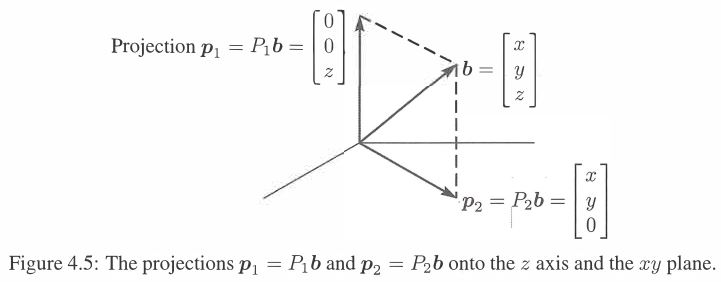
\includegraphics[scale=0.7]{Pro.JPG}
\end{figure}
\begin{itemize}
    \item The projection onto the $z$ axis denoted $p_1$:
    \begin{figure} [h!]
        \centering
        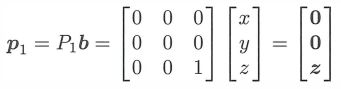
\includegraphics[scale=0.6]{p1.JPG}
    \end{figure}
    \item The projection onto the $xy$ axis denoted $p_2$:
    \begin{figure} [h!]
        \centering
        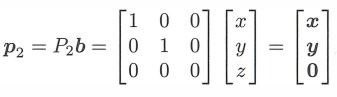
\includegraphics[scale=0.6]{p2.JPG}
    \end{figure}
\end{itemize}
where the \textbf{projection matrix} extracts the wanted components from $b$.

Note that the two projected lines $p_1$ and $p_2$ are orthogonal complements. Their dimensions add
to $1  +  2  =  3$. Every vector $b$ in the whole space is the sum of its parts in the two
subspaces, for example the projections $p_1$ and $p_2$ are exactly those two parts of $b$.

\pagebreak

This example shows the objective: find the part $p$ in each subspace, and the projection matrix $P$
that produces that part $p = Pb$.  

Every subspace of $R^m$ has its own $[m\times m]$ projection matrix. To compute $P$, a good
description of the subspace that it projects onto is needed. The best description of a subspace is a
basis.

%%%%%%%%%%%%%%%%%%%%%%%%%%%%%%%%%%%%%%%%%%%%%%%%%%%%%%%%%%%%%%%%%%%%%%%%%%%%%%%%%%%%%%%%%%%%%%%%%%%%%%%%%%
\subsubsection{Projection onto 1D}

The key to projection is orthogonality and it well known that the perpendicular distance is the
shortest distance between two lines. In estimation, it is of interest the point given by
$\textbf{\underline{p}}$ i.e. the projection of $\textbf{\underline{b}}$ onto
$\textbf{\underline{a}}$. \textbf{The line from $b$ to $p$ is perpendicular to $a$}

The particular reason is that this is the point on $\textbf{\underline{a}}$ nearest to
$\textbf{\underline{b}}$. Recall the usual objective is to obtain $\textbf{\underline{b}}$, but this
is not available, thus to points on $\textbf{\underline{a}}$, the nearest point on
$\textbf{\underline{a}}$ is the projection $\textbf{\underline{p}}$. 

The projection $\textbf{\underline{p}}$ will be some multiple of $\textbf{\underline{a}}$:
\begin{align*}
    \textbf{\underline{p}} = \hat{\textbf{\underline{x}}} \times \textbf{\underline{a}}
\end{align*}    
These three steps will lead to all projection matrices: 
\begin{itemize}
    \item Find $\hat{\textbf{\underline{x}}}$
    \begin{align*}
        \hat{\textbf{\underline{x}}} = \frac{\textbf{\underline{a}}.\textbf{\underline{b}}}{\textbf{\underline{a}}.\textbf{\underline{a}}} = \frac{\textbf{\underline{a}}^T \textbf{\underline{b}}}{\textbf{\underline{a}}^T \textbf{\underline{a}}}
    \end{align*}
    \item Computing $\hat{\textbf{\underline{x}}}$ will give the vector $\textbf{\underline{p}}$
    \begin{align*}
        \textbf{\underline{p}} = \frac{\textbf{\underline{a}}^T \textbf{\underline{b}}}{\textbf{\underline{a}}^T \textbf{\underline{a}}} \textbf{\underline{a}} = \frac{\textbf{\underline{a}} \textbf{\underline{a}}^T}{\textbf{\underline{a}}^T \textbf{\underline{a}}} \textbf{\underline{b}} 
    \end{align*}
    where $(\textbf{\underline{a}}^T \textbf{\underline{b}})\textbf{\underline{a}}=\textbf{\underline{a}}(\textbf{\underline{a}}^T\textbf{\underline{b}})$
    \item From the formula for $\textbf{\underline{p}}$, the projection matrix $P$ can be found
    \begin{align*}
        P = \frac{\textbf{\underline{a}} \textbf{\underline{a}}^T}{\textbf{\underline{a}}^T \textbf{\underline{a}}}
    \end{align*}
\end{itemize}
\begin{figure} [h!]
    \centering
    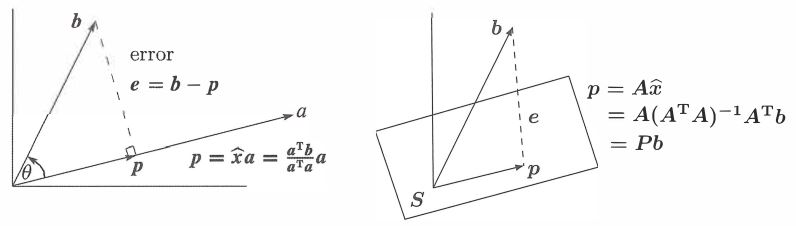
\includegraphics[scale=0.6]{proj.JPG}
    \caption{The projection $p$ of $b$ onto a line and onto $S =$ column space of $A$}
\end{figure}

\pagebreak

Note that if projection occurs twice onto $\textbf{\underline{a}}$? The first time from
$\textbf{\underline{b}}$ to $\textbf{\underline{p}}$ but the second time - nothing happens. This is
due to that there is a line through $\textbf{\underline{a}}$ already.
\begin{align*}
    P^2 \textbf{\underline{b}} = P(P\textbf{\underline{b}}) = P\textbf{\underline{p}} = \textbf{\underline{p}} = P\textbf{\underline{b}}
\end{align*}

The difference real and approximation becomes the resulting error $\textbf{\underline{e}} \neq 0$.
\begin{align*}
    \textbf{\underline{e}} = \textbf{\underline{b}} - \hat{\textbf{\underline{x}}}\textbf{\underline{a}}
\end{align*}

%%%%%%%%%%%%%%%%%%%%%%%%%%%%%%%%%%%%%%%%%%%%%%%%%%%%%%%%%%%%%%%%%%%%%%%%%%%%%%%%%%%%%%%%%%%%%%%%%%%%%%%%%%
\subsubsection{Projection onto 2D}

Returning to the problem $A\textbf{\underline{x}} = \textbf{\underline{b}}$ which has no solution.
To find the closest thing to a solution:
\begin{itemize}
    \item Consider that $A\textbf{\underline{x}}$ is in the column
    space of $C(A)$, and look for $\textbf{\underline{p}}$ which is the closest vector in $C(A)$ to
    $\textbf{\underline{b}}$
    \item Solve $A\hat{\textbf{\underline{x}}} = \textbf{\underline{p}}$ where $\textbf{\underline{p}}$ is the projection of $\textbf{\underline{b}}$ onto the column
    space of $A$.
    \begin{align*}
        A^T A \hat{\textbf{\underline{x}}} = A^T \textbf{\underline{b}}
    \end{align*}
\end{itemize}
\begin{figure} [h!]
    \centering
    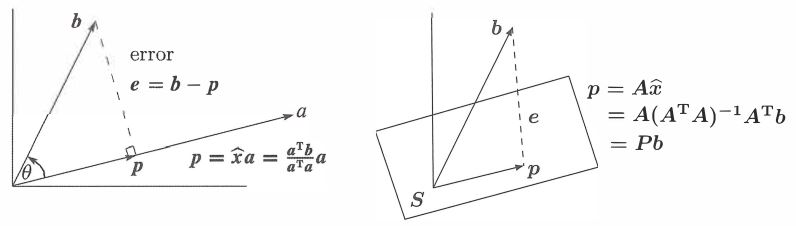
\includegraphics[scale=0.6]{proj.JPG}
    \caption{The projection $p$ of $b$ onto a line and onto $S =$ column space of $A$}
\end{figure}

The steps is the same as the previous topic.
These three steps will lead to all projection matrices: 
\begin{itemize}
    \item Find $\hat{\textbf{\underline{x}}}$
    \begin{align*}
        \hat{\textbf{\underline{x}}} = (A^T A)^{-1}A^T \textbf{\underline{b}} = \frac{\textbf{\underline{a}}.\textbf{\underline{b}}}{\textbf{\underline{a}}.\textbf{\underline{a}}} = \frac{\textbf{\underline{a}}^T \textbf{\underline{b}}}{\textbf{\underline{a}}^T \textbf{\underline{a}}}
    \end{align*}
    \item Computing $\hat{\textbf{\underline{x}}}$ will give the vector $\textbf{\underline{p}}$
    \begin{align*}
        \textbf{\underline{p}} = A\hat{\textbf{\underline{x}}} = A(A^T A)^{-1}A^T \textbf{\underline{b}} = \frac{\textbf{\underline{a}}^T \textbf{\underline{b}}}{\textbf{\underline{a}}^T \textbf{\underline{a}}} \textbf{\underline{a}} = \frac{\textbf{\underline{a}} \textbf{\underline{a}}^T}{\textbf{\underline{a}}^T \textbf{\underline{a}}} \textbf{\underline{b}} 
    \end{align*}
    where $(\textbf{\underline{a}}^T \textbf{\underline{b}})\textbf{\underline{a}}=\textbf{\underline{a}}(\textbf{\underline{a}}^T\textbf{\underline{b}})$
    \item From the formula for $\textbf{\underline{p}}$, the projection matrix $P$ can be found
    \begin{align*}
        P = A(A^T A)^{-1} A^T = \frac{\textbf{\underline{a}} \textbf{\underline{a}}^T}{\textbf{\underline{a}}^T \textbf{\underline{a}}}
    \end{align*}
\end{itemize}

\pagebreak

Note that the projection matrix had two properties:
\begin{itemize}
    \item $P$ is symmetric
    \item $P^2 = P$
\end{itemize}

\pagebreak

%%%%%%%%%%%%%%%%%%%%%%%%%%%%%%%%%%%%%%%%%%%%%%%%%%%%%%%%%%%%%%%%%%%%%%%%%%%%%%%%%%%%%%%%%%%%%%%%%%%%%%%%%%
\section{Least-squares method or Linear Regression}

It often happens that $A\textbf{\underline{x}} = \textbf{\underline{b}}$ has no solution. The usual
reason is: too many equations. The matrix $A$ has more rows than columns. There are more equations
than unknowns i.e $m$ is greater than $n$. 

When $A\textbf{\underline{x}} = \textbf{\underline{b}}$ has no solution, multiply by $A^T$ and solve
$A^T A \textbf{\underline{x}} = A^T \textbf{\underline{b}}$. A crucial application of least squares
is fitting a straight line to $m$ points.

\textbf{Worked Example}: Find the closest line to the points $(0, 6)$, $(1, 0)$, and $(2, 0)$. 

No straight line $b =  C + Dt$ goes through those three points. We are asking for two numbers $C$
and $D$ that satisfy three equations from the three coordinates listed.  

Here are the three equations at $t = 0$, $1$, $2$ to match the given values $\textbf{\underline{b}} = 6, 0, 0$: 
\begin{align*}
    C + D.0 = 6 \\
    C + D.1 = 0 \\
    C + D.2 = 0
\end{align*}

Notice that this 3 by 2 system has no solution: $\textbf{\underline{b}} = 6, 0, 0$ is not a
combination of the columns $(1, 1, 1)$ and $(0, 1, 2)$:
\begin{align*}
    A\textbf{\underline{x}} = \textbf{\underline{b}} \Rightarrow \begin{pmatrix}
        1&0 \\
        1&1 \\
        1&2
    \end{pmatrix}\begin{pmatrix}
        C \\ D
    \end{pmatrix} = \begin{pmatrix}
        6\\0\\0
    \end{pmatrix}
\end{align*}

To find the best fit solution, solve $A^T A \hat{\textbf{\underline{x}}} = A^T
\textbf{\underline{b}}$: where $\hat{\textbf{\underline{x}}} =
\begin{pmatrix}\hat{C}\\\hat{D}\end{pmatrix}$ will be the "best" approximations to the impossible
$\begin{pmatrix}C\\D\end{pmatrix}$.
\begin{align*}
    A^T A \hat{\textbf{\underline{x}}} = \textbf{\underline{b}} &\Rightarrow \begin{pmatrix} 
        1&1&1\\
        0&1&2
    \end{pmatrix}\begin{pmatrix}
        1&0\\1&1\\1&2
    \end{pmatrix}\hat{\textbf{\underline{x}}} = \begin{pmatrix} 
        1&1&1\\
        0&1&2
    \end{pmatrix}\begin{pmatrix}
        6\\0\\0
    \end{pmatrix}  \\
    &= \begin{pmatrix}
        3&3 \\ 3&5
    \end{pmatrix}\begin{pmatrix}
        \hat{C} \\
        \hat{D}
    \end{pmatrix} = \begin{pmatrix}
        6\\0
    \end{pmatrix}
\end{align*}

Solve the two equations to find the values of $\hat{C}$ and $\hat{D}$.
\begin{align*}
    3\hat{C} + 3\hat{D} = 6 \\
    3\hat{C} + 5\hat{D} = 0 
\end{align*}
Thus:
\begin{align*}
    \hat{\textbf{\underline{x}}} = \begin{pmatrix}
        \hat{C} \\ \hat{D}
    \end{pmatrix} = \begin{pmatrix}
        5 \\ -3
    \end{pmatrix}
\end{align*}

\pagebreak

So the though least square approximation, the points closest to $\textbf{\underline{b}}$ denoted $\hat{\textbf{\underline{b}}}$ is found:
\begin{align*}
    A \hat{\textbf{\underline{x}}} = \hat{\textbf{\underline{b}}} &\Rightarrow \begin{pmatrix}
        1&0 \\
        1&1 \\
        1&2
    \end{pmatrix}\begin{pmatrix}
        5\\-3
    \end{pmatrix} \\
    &= \begin{pmatrix}
        5 \\ 2 \\ -1
    \end{pmatrix}
\end{align*}

%%%%%%%%%%%%%%%%%%%%%%%%%%%%%%%%%%%%%%%%%%%%%%%%%%%%%%%%%%%%%%%%%%%%%%%%%%%%%%%%%%%%%%%%%%%%%%%%%%%%%%%%%%
\subsection{Minimising error}

How do we make the error $\textbf{\underline{e}} = \textbf{\underline{b}} - A\hat{\textbf{\underline{x}}}$ as small as possible? Recall that the point nearest to $b$ is
basically the projection $p$.

The smallest possible error is perpendicular to the columns defined as:
\begin{align*}
    \textbf{\underline{e}} = \textbf{\underline{b}} - \textbf{\underline{p}}
\end{align*}
 
%%%%%%%%%%%%%%%%%%%%%%%%%%%%%%%%%%%%%%%%%%%%%%%%%%%%%%%%%%%%%%%%%%%%%%%%%%%%%%%%%%%%%%%%%%%%%%%%%%%%%%%%%%
\pagebreak
%%%%%%%%%%%%%%%%%%%%%%%%%%%%%%%%%%%%%%%%%%%%%%%%%%%%%%%%%%%%%%%%%%%%%%%%%%%%%%%%%%%%%%%%%%%%%%%%%%%%%%%%%%
\section{Orthogonality and QR}

There are two objective to this section:
\begin{itemize}
    \item The first is to see why orthogonality is good.
    \item The second goal is to construct the orthogonal vectors.
\end{itemize} 

Dot products are zero, so $A^T A$ will be diagonal. It becomes so easy to find
$\hat{\textbf{\underline{x}}}$ and $\textbf{\underline{p}} = A\hat{\textbf{\underline{x}}}$. 

Orthogonal vectors are constructed from the Gram-Schmidt process which chooses combinations of the original basis vectors to produce right angles.

%%%%%%%%%%%%%%%%%%%%%%%%%%%%%%%%%%%%%%%%%%%%%%%%%%%%%%%%%%%%%%%%%%%%%%%%%%%%%%%%%%%%%%%%%%%%%%%%%%%%%%%%%%
\subsection{Orthonormal vectors and orthogonal matrices}

Recall that a basis consists of independent vectors that span the space. The basis vectors could
meet at any angle except at 0 and 180.

The vectors $q_1,\dots,q_n$ are orthogonal when their dot products $q_i.q_j$ are zero i.e. $q_i^Tq_j
= 0$ whenever $i \neq j$. The \textbf{orthogonal unit vectors} are found by dividing each vector by
its length.

\begin{tcolorbox}[breakable,colback=white]
\textbf{Orthonomality}: A matrix with orthonormal columns is assigned the special letter $Q$. 
\begin{align*}
    \boldsymbol{q}_{i}^{\mathrm{T}} \boldsymbol{q}_{j}=\left\{\begin{array}{ll}
        0 & \text { when } i \neq j \quad \text { (orthogonal vectors) } \\
        1 & \text { when } i=j \quad\left(\text {unit vectors: }\left\|\boldsymbol{q}_{i}\right\|=1\right)
        \end{array}\right.
\end{align*}
\end{tcolorbox}

The reason for $Q$ is because it is easy to work with since $Q^T  Q  = I$. A matrix $Q$ with
orthonormal columns satisfies $Q^TQ=I$:
\begin{align*}
    \boldsymbol{Q}^{\mathrm{T}} \boldsymbol{Q}=\left[\begin{array}{l}
        -\boldsymbol{q}_{1}^{\mathrm{T}}- \\
        -\boldsymbol{q}_{2}^{\mathrm{T}}- \\
        -\boldsymbol{q}_{n}^{\mathrm{T}}-
        \end{array}\right]\left[\begin{array}{ccc}
        \mid & \mid & \mathbf{1} \\
        \boldsymbol{q}_{1} & \boldsymbol{q}_{2} & \boldsymbol{q}_{n} \\
        \mid & \mid & \vdots
        \end{array}\right]=\left[\begin{array}{cccc}
        1 & 0 & \cdots & 0 \\
        0 & 1 & \cdots & 0 \\
        \vdots & \vdots & \ddots & \vdots \\
        0 & 0 & \cdots & 1
        \end{array}\right]=I
\end{align*}

\begin{tcolorbox}[breakable,colback=white]
    When $Q$ is square, $Q^T Q  = I$ means that $Q^T = Q^{-1}$ i.e. transpose = inverse. In this
    case, $Q$ is an \textbf{orthogonal matrix}. 
\end{tcolorbox}

\pagebreak

\textbf{Example 1}: Check if the given matrix $Q = \begin{pmatrix}
    1&1\\-1&1
\end{pmatrix}$ is orthogonal or not.

Matrix $Q$ is almost orthogonal, it needs to be normalised first:
\begin{align*}
    \hat{Q} = \frac{1}{\sqrt{2}} \begin{pmatrix}
        1&1\\-1&1
    \end{pmatrix}
\end{align*}

Normalised matrix $Q$ satisfies the orthogonality property:
\begin{align*}
    Q \times Q^T = \begin{pmatrix}
        \frac{1}{\sqrt{2}}&\frac{1}{\sqrt{2}} \\
        -\frac{1}{\sqrt{2}}&\frac{1}{\sqrt{2}}
    \end{pmatrix} \times \begin{pmatrix}
        \frac{1}{\sqrt{2}}&-\frac{1}{\sqrt{2}} \\
        \frac{1}{\sqrt{2}}&\frac{1}{\sqrt{2}}
    \end{pmatrix} = \begin{pmatrix}
        1&0\\0&1
    \end{pmatrix}
\end{align*}

Note that rotations preserve the length of every vector. So do reflections. So do permutations. 
So does multiplication by any orthogonal matrix $Q$ i.e. lengths and angles don't change.

\begin{tcolorbox}[breakable,colback=white]
    If $Q$ has orthonormal columns ($Q^T Q = I$), it leaves lengths unchanged:
    \begin{align*}
        ||Q \textbf{x}|| = ||\textbf{x}||
    \end{align*}

    This means that $Q$ also preserves dot products:
    \begin{align*}
        (Q \textbf{x})^T(Q \textbf{y}) = \textbf{x}^TQ^TQ\textbf{y} = \textbf{x}^T\textbf{y}
    \end{align*}
    thus simplifying to
    \begin{align*}
        Q^TQ = I
    \end{align*}
\end{tcolorbox}

%%%%%%%%%%%%%%%%%%%%%%%%%%%%%%%%%%%%%%%%%%%%%%%%%%%%%%%%%%%%%%%%%%%%%%%%%%%%%%%%%%%%%%%%%%%%%%%%%%%%%%%%%%
\subsubsection{Projections Using Orthonormal Bases: $Q$ replaces $A$}

Recall:
\begin{itemize}
    \item How a projection works: we would like to project onto the column space of a matrix, as we
    did, for example, in the least-squares algorithm. 
    \item A system of linear equations $A\textbf{\underline{x}} = \textbf{\underline{b}}$ has no
    solution, but we can find the nearest point to $\textbf{\underline{b}}$ in the column space of $A$,
    so that $A^T A \hat{\textbf{\underline{x}}} = A^T \textbf{\underline{b}}$ does have a solution.
\end{itemize}

Suppose the basis vectors are actually orthonormal. Then $A^T A$ simplifies to $Q^T Q = I$. This
means that the least squares solution of $Qx = b$ is $x = Q^T b$ and the projection matrix is $QQ^T$. 

There are no matrices to invert. This is the point of an orthonormal basis. The best $\textbf{\underline{x}} = 
Q^T \textbf{\underline{b}}$ just has dot products of $q_1,\dots,q_n$ with $\textbf{\underline{b}}$.
The result is 1-dimensional projections.

\pagebreak

%%%%%%%%%%%%%%%%%%%%%%%%%%%%%%%%%%%%%%%%%%%%%%%%%%%%%%%%%%%%%%%%%%%%%%%%%%%%%%%%%%%%%%%%%%%%%%%%%%%%%%%%%%
\subsection{Gram-Schmidt process}

The immense benefit of using $Q$ has already been stated and all these relies on the fact that the
\textbf{basis are orthonormal}. The Gram-Schmidt process is a way to create these orthonormal
vectors.

Start with three \textbf{independent} vectors $a$, $b$, $c$. We intend to construct three orthogonal vectors
$A$, $B$, $C$. Then we divide $A$, $B$, $C$ by their lengths, this produces three orthonormal 
vectors $q_1  = \frac{A}{||A||}$,  $q_2  = \frac{b}{||b||}$, $q_3 = \frac{C}{||C||}$.

Begin by choosing $A = \textbf{a}$. This first direction does not really matter and can be accepted as it comes. 
The next direction $B$ \textbf{must be perpendicular to $A$}. Start with $\textbf{b}$ and subtract
its projection along $A$ - leaving the perpendicular part, which is the orthogonal vector $B$:
\begin{align}
    B = \textbf{b} - \frac{A^T \textbf{b}}{A^T A} A
\end{align}

$A$ and $B$ are orthogonal now.

The third direction starts with $c$. This is not a combination of $A$ and $B$ (because $c$ is not a
combination of $a$ and $b$). $c$ is not perpendicular to $A$ and $B$ so subtract off its components
in those two directions to get a perpendicular direction $C$:
\begin{align}
    C = \textbf{c} - \frac{A^T \textbf{c}}{A^T A} A - \frac{B^T \textbf{c}}{B^T B} B
\end{align}

The Gram-Schmidt process can be summarised as: \textit{Subtract from every new vector its
projections in the directions already set}.

At the end, or immediately when each one is found, divide the orthogonal vectors $A$, $B$, $C$ by
their lengths. The resulting vectors $q_1$, $q_2$, $q_3$ are orthonormal.

\textbf{Example 1}: Consider the basis of $\Re^3$
\begin{align*}
    \textbf{a} = \begin{bmatrix}
        1\\2\\0
    \end{bmatrix} \; \textbf{b} = \begin{bmatrix}
        1\\1\\1
    \end{bmatrix} \; \textbf{c} = \begin{bmatrix}
        1\\2\\3
    \end{bmatrix}
\end{align*}
Obtain an orthonormal basis by implementing the Gram-Schmidt process.

\begin{enumerate}
    \item $A$:
    \begin{align*}
        A = \begin{bmatrix}
            1\\2\\0
        \end{bmatrix}
    \end{align*}

    \item $B$:
    \begin{align*}
        B = \textbf{b} - \frac{A^T \textbf{b}}{A^T A} A = \begin{bmatrix}
            1\\1\\1
        \end{bmatrix} - \frac{3}{5} \begin{bmatrix}
            1\\2\\0
        \end{bmatrix} = \frac{1}{5}\begin{bmatrix}
            2\\-1\\5
        \end{bmatrix}
    \end{align*}

    \pagebreak

    Note that both $\frac{1}{5}\begin{bmatrix}
        2\\-1\\5
    \end{bmatrix}$ and $\begin{bmatrix}
        2\\-1\\5
    \end{bmatrix}$ are clearly orthogonal so $B$ can be simplified to $B = \begin{bmatrix}
        2\\-1\\5
    \end{bmatrix}$.

    \item $C$: 
    \begin{align*}
        C = \textbf{c} - \frac{A^T \textbf{c}}{A^T A} A - \frac{B^T \textbf{c}}{B^T B} B = \left[\begin{array}{l}
            1 \\
            2 \\
            3
            \end{array}\right]-\frac{15}{30}\left[\begin{array}{r}
            2 \\
            -1 \\
            5
            \end{array}\right]-\frac{5}{5}\left[\begin{array}{l}
            1 \\
            2 \\
            0
            \end{array}\right]=\frac{1}{2}\left[\begin{array}{r}
            -2 \\
            1 \\
            1
            \end{array}\right]
    \end{align*}
\end{enumerate}

To get an orthonormal basis, divide each vector by its length:
\begin{align*}
    \begin{array}{l}
        A=\frac{1}{\left\|\underline{\mathbf{x}}_{1}\right\|} \underline{\mathbf{x}}_{1}=\frac{1}{\sqrt{5}}\left[\begin{array}{l}
        1 \\
        2 \\
        0
        \end{array}\right] \\
        B=\frac{1}{\left\|\underline{\mathbf{x}}_{2}\right\|} \underline{\mathbf{x}}_{2}=\frac{1}{\sqrt{30}}\left[\begin{array}{r}
        2 \\
        -1 \\
        5
        \end{array}\right] \\
        C=\frac{1}{\left\|\underline{\mathbf{x}}_{3}\right\|} \underline{\mathbf{x}}_{3}=\frac{1}{\sqrt{6}}\left[\begin{array}{r}
        -2 \\
        1 \\
        1
        \end{array}\right]
    \end{array}
\end{align*}

\pagebreak

%%%%%%%%%%%%%%%%%%%%%%%%%%%%%%%%%%%%%%%%%%%%%%%%%%%%%%%%%%%%%%%%%%%%%%%%%%%%%%%%%%%%%%%%%%%%%%%%%%%%%%%%%%
\subsection{Factorization $A = QR$}

We started with a matrix $A$,  whose columns  were  $\textbf{a}$, $\textbf{b}$ and $\textbf{c}$.
Through the Gram-Schmidt process, a matrix $Q$ is formed from the independent vectors
$\textbf{q}_1$, $\textbf{q}_2$, $\textbf{q}_3$. This hints that there must be a relationship between
the two matrices.

Given the relations between the columns of $A$ and $Q$, we can write these as a matrix product:
\begin{align*}
    A = QR
\end{align*}

Note the key points of Gram-Schmidt:
\begin{itemize}
    \item The vectors $\textbf{a}$ and $A$ and $\textbf{q}_1$ are all along a single line. This
    means that $\textbf{q}_1$ is a linear combination of $\textbf{a}$.
    \item The vectors $\textbf{a}$, $\textbf{b}$ and $A$, $B$ and $\textbf{q}_1$, $\textbf{q}_2$ are
    all in the same plane. This means that $\textbf{q}_2$ is a linear combination of $\textbf{a}$ and $\textbf{b}$.
    \item The vectors $\textbf{a}$, $\textbf{b}$, $\textbf{c}$ and $A$, $B$, $C$ and $\textbf{q}_1$,
    $\textbf{q}_2$, $\textbf{q}_3$ are in one subspace (dimension 3). Note that $\textbf{q}_3$ is
    orthogonal to $\textbf{q}_1$ and $\textbf{q}_2$ thus also orthogonal to $\textbf{a}$ and $\textbf{b}$.
\end{itemize} 

$A = QR$ is Gram-Schmidt in a nutshell:
\begin{align*}
    \left[\begin{array}{lll}
        a & b & c
        \end{array}\right]=\left[\begin{array}{lll}
        q_{1} & q_{2} & q_{3}
        \end{array}\right]\left[\begin{array}{lll}
        q_{1}^{\mathrm{T}} a & q_{1}^{\mathrm{T}} b & q_{1}^{\mathrm{T}} c \\
        & q_{2}^{\mathrm{T}} b & q_{2}^{\mathrm{T}} c \\
        & & q_{3}^{\mathrm{T}} c
        \end{array}\right]
\end{align*}

Multiply by $Q^T$ to recognize $R = Q^T A$:
\begin{align*}
    R=Q^{T} A &= \begin{bmatrix}
        \underline{\mathbf{q}}_{1}^{T} \\
        \underline{\mathbf{q}}_{2}^{T} \\
        \underline{\mathbf{q}}_{3}^{T}
    \end{bmatrix}
    \begin{bmatrix}
        \underline{\mathrm{a}}_{1}&\underline{\mathrm{a}}_{2}&\underline{\mathrm{a}}_{3}
    \end{bmatrix} \\ &= 
    \begin{bmatrix}
        \underline{\mathbf{q}}_{1}^{T} \underline{\mathbf{a}}_{1} & \underline{\mathbf{q}}_{1}^{T} \underline{\mathbf{a}}_{2} & \underline{\mathbf{q}}_{1}^{T} \underline{\mathbf{a}}_{3} \\
        \underline{\mathbf{q}}_{2}^{T} \underline{\mathbf{a}}_{1} & \underline{\mathbf{q}}_{2}^{T} \underline{\mathbf{a}}_{2} & \underline{\mathbf{q}}_{2}^{T} \underline{\mathbf{a}_{3}} \\
        \underline{\mathbf{q}}_{3}^{T} \underline{\mathbf{a}}_{1} & \underline{\mathbf{q}}_{3}^{T} \underline{\mathbf{a}}_{2} & \underline{\mathbf{q}}_{3}^{T} \underline{\mathbf{a}}_{3}
    \end{bmatrix} \\ &= 
    \begin{bmatrix}
        \mathbf{q}_{1}^{T} \mathbf{a}_{1} & \underline{\mathbf{q}}_{1}^{T} \underline{\mathbf{a}}_{2} & \underline{\mathbf{q}}_{1}^{T} \underline{\mathbf{a}}_{3} \\
        0 & \underline{\mathbf{q}}_{2}^{T} \underline{\mathbf{a}}_{2} & \underline{\mathbf{q}}_{2}^{T} \underline{\mathbf{a}}_{3} \\
        0 & 0 & \underline{\mathbf{q}}_{3}^{T} \underline{\mathbf{a}}_{3}
    \end{bmatrix} 
\end{align*}

\pagebreak

\textbf{Example 1}: Given the $3 \times 2$ "tall" matrix:
\begin{align*}
    A=\left(\begin{array}{cc}
        2 & 1 \\
        3 & 12 \\
        6 & 10
    \end{array}\right)
\end{align*}
obtain the $QR$-factorization.

\begin{itemize}
    \item Consider the size of $R$: $A$ is $3 \times 2$, so $Q$ will be $3 \times 2$ and $R$ will be $2 \times 2$.
    \item Implement least-squares method:
    \begin{itemize}
        \item Set $\textbf{q}_1$ as $\textbf{x}_1$:
        \begin{align*}
            \textbf{q}_1 = \begin{pmatrix}
                2\\3\\6
            \end{pmatrix}
        \end{align*}
        \item Find $\textbf{q}_2$:
        \begin{align*}
            \underline{\mathbf{c}}_{2}-\frac{\underline{\mathbf{q}}_{1}^{T} \underline{\mathbf{c}}_{2}}{\underline{\mathbf{q}}_{1}^{T} \underline{\mathbf{q}}_{1}} \underline{\mathbf{q}}_{1}=\left(\begin{array}{c}
                1 \\
                12 \\
                10
                \end{array}\right)-\frac{2+36+60}{4+9+36}\left(\begin{array}{c}
                2 \\
                3 \\
                6
                \end{array}\right)=\left(\begin{array}{c}
                -3 \\
                6 \\
                -2
                \end{array}\right)
        \end{align*}
        \item Normalization:
        \begin{align*}
            Q=\frac{1}{7}\left(\begin{array}{cc}
                2 & -3 \\
                3 & 6 \\
                6 & -2
                \end{array}\right)
        \end{align*}
    \end{itemize}
    \item Find $R$ by using $R = Q^TA$:
    \begin{align*}
        Q^{T} A&=Q^{T}(Q R)=R \\ &\Longrightarrow\left(\begin{array}{c}
            \underline{\mathbf{q}}_{1}^{T} \\
            \underline{\mathbf{q}}_{2}^{T}
            \end{array}\right)\left(\begin{array}{cc}
            \mathbf{c}_{1} \mathbf{c}_{2}
            \end{array}\right)=\left(\begin{array}{cc}
            \underline{\mathbf{q}}_{1}^{T} \mathbf{c} 1 & \underline{\mathbf{q}}_{1}^{T} \underline{\mathbf{c}}_{2} \\
            0 & \underline{\mathbf{q}}_{2}^{T} \underline{\mathbf{c}}_{2}
            \end{array}\right)=\left(\begin{array}{cc}
            7 & 14 \\
            0 & 7
            \end{array}\right)
    \end{align*}
\end{itemize}

\pagebreak

The critical part of this chapter. Recall how we the method of least-squares relied on a matrix $A$
with independent columns:
\begin{align*}
    A^{T} A \underline{\hat{x}}=A^{T} \underline{\mathbf{b}}
\end{align*}
Now, with $A = QR$ - factorization we can write:
\begin{align*}
    A^{T} A=(Q R)^{T} Q R=\left(R^{T} Q^{T}\right)(Q R)=R^{T}\left(Q^{T} Q\right) R=R^{T} R
\end{align*}
as $Q^T Q = I$, thus the problem becomes the need to solve:
\begin{align*}
    R^{T} R \underline{\hat{\mathbf{x}}}=R^{T} Q^{T} \underline{\mathbf{b}}
\end{align*}
Having established earlier that $A^T A$ is invertible, and therefore $R^T R = A^T A$ is also
invertible. This means that we can multiply by $(R^{T})^{-1}$:
\begin{align*}
    R \underline{\hat{x}}&=Q^{T} \underline{\mathbf{b}} \\
    \widehat{\boldsymbol{x}}&=R^{-1} Q^{\mathrm{T}} \boldsymbol{b}
\end{align*}

\pagebreak

%%%%%%%%%%%%%%%%%%%%%%%%%%%%%%%%%%%%%%%%%%%%%%%%%%%%%%%%%%%%%%%%%%%%%%%%%%%%%%%%%%%%%%%%%%%%%%%%%%%%%%%%%%
\section{Eigenvalues, Eigenvectors and Diagonalisation}

The first part was about $Ax  =  b$: balance and equilibrium and steady state. Now the second part
is about change i.e. time enters the picture-continuous time in a differential equation or time
steps in a difference equation. Those equations cannot be solved by elimination. 

The key idea to solving these equations is to avoid all the complications presented by the matrix
$A$. We want "eigenvectors" $\textbf{x}$ that don't change direction when you multiply by $A$. A
good example comes from the powers $A$, $A^2$, $A^3$,\dots of a matrix. 

Suppose you need $A^{100}$. Its columns are very close to the eigenvector $( .6,  .4)$: 
\begin{figure} [h!]
    \centering
    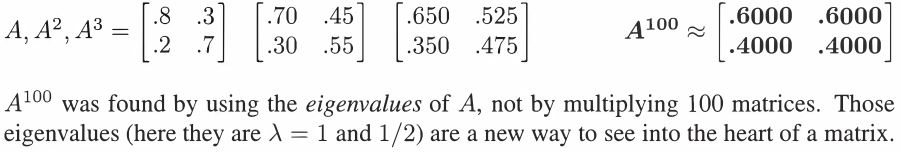
\includegraphics[scale=0.6]{Line.JPG}
\end{figure}

%%%%%%%%%%%%%%%%%%%%%%%%%%%%%%%%%%%%%%%%%%%%%%%%%%%%%%%%%%%%%%%%%%%%%%%%%%%%%%%%%%%%%%%%%%%%%%%%%%%%%%%%%%
\subsection{Eigenvectors}

Almost all vectors change direction when multiplied by $A$. Certain exceptional vectors $\textbf{x}$
are in the same direction as $A \textbf{x}$. Those are the "eigenvectors" - Multiply an eigenvector by $A$,
and the vector $A \textbf{x}$ is a number $\lambda$ times the original $\textbf{x}$. 
\begin{align*}
    \text{The basic equation is } A \textbf{x} = \lambda \textbf{x} \; \text{ where } \lambda \text{ is an eigenvalue of } A 
\end{align*}
The eigenvalue $\lambda$ tells whether the special vector $\textbf{x}$ is stretched or shrunk or reversed or left
unchanged when multiplied by $A$. Recall that a $\lambda$ value of 0 then $A \textbf{x} = O \textbf{x}$ means that this eigenvector is in the nullspace. 



%%%%%%%%%%%%%%%%%%%%%%%%%%%%%%%%%%%%%%%%%%%%%%%%%%%%%%%%%%%%%%%%%%%%%%%%%%%%%%%%%%%%%%%%%%%%%%%%%%%%%%%%%%
\subsection{Solving the Eigenvalue Equation}

\begin{tcolorbox}[breakable,colback=white]
    \textbf{Characteristic polynomial} of the matrix $A$: 
    \begin{align*}
        P_A(\lambda) = \text{det}(A-\lambda I)
    \end{align*}

    \textbf{Characteristic equation}: 
    \begin{align*}
    \text{det}(A-\lambda I) = 0
    \end{align*}
\end{tcolorbox}

\pagebreak

This gives the algorithm: to find the eigenvalues and eigenvectors of a matrix $A$:
\begin{enumerate}
    \item Fnd all scalars $\lambda$ that are zeros of the characteristic equation to find the eigenvalues:
    \begin{align*}
        P_A(\lambda) = \text{det}(A-\lambda I) = 0
    \end{align*}

    \item For each such $\lambda$, find a non-zero solution of the equation to derive the corresponding eigenvectors:
    \begin{align*}
        (A - \lambda I)\textbf{\underline{x}} = \textbf{\underline{0}}
    \end{align*}
\end{enumerate}

\textbf{Example 1}: Find eigenvalues and eigenvectors of the matrix
\begin{align*}
    A = \begin{pmatrix}
        2&1 \\ 1&2
    \end{pmatrix}
\end{align*}
\begin{itemize}
    \item Begin with the characteristic equation:
    \begin{align*}
        A-\lambda I&=\left(\begin{array}{ll}
            2 & 1 \\
            1 & 2
            \end{array}\right)-\lambda\left(\begin{array}{ll}
            1 & 0 \\
            0 & 1
            \end{array}\right)=\left(\begin{array}{cc}
            2-\lambda & 1 \\
            1 & 2-\lambda
            \end{array}\right) \\
            &\Longrightarrow \operatorname{det}(A-\lambda I)=(2-\lambda)(2-\lambda)-1=0
    \end{align*}
    solutions $\lambda = 3 \text{ and } 1$.

    \item To find the eigenvectors, solve $(A - \lambda I)\textbf{\underline{x}} =
    \textbf{\underline{0}}$ for each eigenvalue.
    \begin{itemize}
        \item $\lambda = 3$:
        \begin{align*}
            A-3 I=\left(\begin{array}{cc}
                -1 & 1 \\
                1 & -1
                \end{array}\right), \quad \text { and } \quad\left(\begin{array}{cc}
                -1 & 1 \\
                1 & -1
                \end{array}\right) \underline{\mathbf{x}}=\underline{\mathbf{0}}
        \end{align*}
        thus
        \begin{align*}
            \underline{\mathbf{x}}_{1}=\left(\begin{array}{l}
                1 \\
                1
                \end{array}\right)
        \end{align*}
        \item $\lambda = 1$:
        \begin{align*}
            A-I=\left(\begin{array}{ll}
                1 & 1 \\
                1 & 1
                \end{array}\right), \quad \text { and } \quad\left(\begin{array}{ll}
                1 & 1 \\
                1 & 1
                \end{array}\right) \underline{\mathbf{x}}=\underline{\mathbf{0}}
        \end{align*}
        thus
        \begin{align*}
            \underline{\mathbf{x}}_{2}=\left(\begin{array}{l}
                1 \\
                -1
                \end{array}\right)
        \end{align*}
    \end{itemize}
\end{itemize}

\pagebreak

\textbf{Example 2}: Consider a rotation by $\frac{\pi}{2}$, with matrix
\begin{align*}
    R = \begin{pmatrix}
        0&-1 \\ 
        -1&0
    \end{pmatrix}
\end{align*}
and find its eigenvalues and eigenvectors.

\begin{itemize}
    \item $P_A(\lambda) = \text{det}(A-\lambda I) = 0$:
    \begin{align*}
        P_A(\lambda) &= \text{det}(A-\lambda I) \\
        &= \begin{pmatrix}
            -\lambda & -1 \\
            -1 & \lambda
        \end{pmatrix} \\
        &= \lambda^2 + 1 \\
        &\Rightarrow \lambda = \pm i
    \end{align*}

    \item $\lambda = i$:
    \begin{align*}
        R-i I &= \left(\begin{array}{cc}
        -i & -1 \\
        1 & -i
        \end{array}\right) \Rightarrow\left(\begin{array}{cc}
        -i & -1 \\
        1 & -i
        \end{array}\right) \underline{\mathbf{x}}=\underline{\mathbf{0}} \\ 
        \underline{\mathbf{x}}_{1} &= \left(\begin{array}{l}
            i \\
            1
            \end{array}\right)
    \end{align*}

    \item $\lambda = -i$:
    \begin{align*}
        (R+i I) \underline{\mathbf{x}} &= \left(\begin{array}{cc}
            i & -1 \\
            1 & i
            \end{array}\right) \underline{\mathbf{x}}=\underline{\mathbf{0}} \\ 
        \underline{\mathbf{x}}_{2} &= \left(\begin{array}{l}
            1 \\
            i
            \end{array}\right)
    \end{align*}
\end{itemize}




\pagebreak
%%%%%%%%%%%%%%%%%%%%%%%%%%%%%%%%%%%%%%%%%%%%%%%%%%%%%%%%%%%%%%%%%%%%%%%%%%%%%%%%%%%%%%%%%%%%%%%%%%%%%%%%%%
\subsection{Diagonlisation}

When $x$ is an eigenvector, multiplication by $A$ is just multiplication by a number $\lambda$ i.e.
$A \textbf{x} = \lambda \textbf{x}$. All the difficulties of matrices are swept away. Instead of an interconnected 
system, we can follow the eigenvectors separately. The 100th power of a diagonal matrix is easy. 

The matrix $A$ turns into a diagonal matrix $\mathbf{\Lambda}$ when eigenvectors are used properly. This is the
matrix form of the previous chapter.  

\textbf{Diagonalization}: Suppose the $[n\times n]$ matrix $A$ has $n$ linearly independent eigenvectors 
$x_1,...,x_n$. Put them into the columns of an eigenvector matrix $X$. Then $X^{-1} AX$ is the eigenvalue matrix  $\mathbf{\Lambda}$: 
\begin{align*}
    \boldsymbol{X}^{-1} \boldsymbol{A} \boldsymbol{X}=\boldsymbol{\Lambda}=\left[\begin{array}{lll}
        \boldsymbol{\lambda}_{\mathbf{1}} \\
        & \ddots \\
        & & \boldsymbol{\lambda}_{\boldsymbol{n}}
        \end{array}\right]
\end{align*}

This is the diagonalization of $A$ and is available for most matrices.

%%%%%%%%%%%%%%%%%%%%%%%%%%%%%%%%%%%%%%%%%%%%%%%%%%%%%%%%%%%%%%%%%%%%%%%%%%%%%%%%%%%%%%%%%%%%%%%%%%%%%%%%%%
\subsection{Powers of matrices and the exponential matrix}

The simplest use of diagonalization is in obtaining powers of a matrix in a manageable form.

Consider $A = S \mathbf{\Lambda} S^{-1}$ then:
\begin{align*}
    A^2 &= (S \mathbf{\Lambda} S^{-1})(S \mathbf{\Lambda} S^{-1}) \\
    &= S \mathbf{\Lambda} (S^{-1} S) \mathbf{\Lambda} S^{-1} \\
    &= S \mathbf{\Lambda}^2 S^{-1}
\end{align*}
Thus this can be summarised as:
\begin{align*}
    A^k = S \mathbf{\Lambda}^k S^{-1}
\end{align*}

Note that the same concept can be applied to exponentials:
\begin{align*}
    e^A = S e^\mathbf{\Lambda}   S^{-1}
\end{align*}

As each of the exponential series on the diagonal in $e^\mathbf{\Lambda}$ converges, this guarantees
convergence of the infinite series of matrices in $e^A$. This result is important in that it has many
applications for example in systems of coupled ODEs. 

\pagebreak

%%%%%%%%%%%%%%%%%%%%%%%%%%%%%%%%%%%%%%%%%%%%%%%%%%%%%%%%%%%%%%%%%%%%%%%%%%%%%%%%%%%%%%%%%%%%%%%%%%%%%%%%%%
\subsection{Coupled First-Order ODEs}

The matrix exponential can be applied to systems of coupled first-order equations. In systems
control, we often come across such equations:
\begin{align*}
    \dot{x}(t) = Ax(t) + Bu(t) \; \text{ where } x(t_0) = x_0
\end{align*}

The solution commonly takes the form:
\begin{align*}
    x(t) = e^{A(t-t_0)}x_0 + \int_{t_0}^t e^{A(t-\tau)}B u(\tau) d\tau
\end{align*}

Note that the equation actually represents a \textbf{state space model} which describes the
behaviour in a particular space. Thus, $x(t)$ could be a vector of state variables $x = (x_1, x_2,
\dots, x_n)$ and $A$ becoming a $[n\times n]$ matrix. 

For example, consider two state variables $x_1(t)$ and $x_2(t)$. These two state variables has the
following corresponding equations;
\begin{align*}
    \dot{x}_1 = ax_1 + bx_1 + u_1(t) \\
    \dot{x}_2 = ax_2 + bx_2 + u_2(t)
\end{align*}

By setting $u = 0$ to further simplify the equation:
\begin{align*}
    \dot{\textbf{x}} = \begin{pmatrix}
        \dot{x}_1 \\
        \dot{x}_2
    \end{pmatrix} = \begin{pmatrix}
        a&b\\c&d
    \end{pmatrix}\begin{pmatrix}
        x_1\\x_2
    \end{pmatrix} = A \textbf{x}    
\end{align*}

Assuming $A$ can be diagonalized i.e. two, independent eigenvectors, we will have an invertible
matrix $S$ and a diagonal matrix $\mathbf{\Lambda}$ such that:
\begin{align*}
    A = S \mathbf{\Lambda} S^{-1} \; \text{ and } \; \mathbf{\Lambda} = S^{-1}AS
\end{align*}

We now introduce a new vector $\textbf{y(t)}$ which contains the solutions to the state variables e.g.
$x_1(t)$. These new vector variables will satisfy the equation $\dot{y} = \mathbf{\Lambda}
\textbf{y}$. 

These vectors are related. Consider the substitution $\textbf{x} = S \textbf{y}$: 
\begin{align*}
    \dot{x} &= S\dot{y} \\
    &= S(\mathbf{\Lambda} \textbf{y}) \\
    &= S(S^{-1}AS)\textbf{y} \\
    &= A(S \textbf{y}) \\
    &= A \textbf{x}
\end{align*}

This means that $\textbf{x} = S \textbf{y}$ is the solution to the system which only requires
finding the eigenvalues and eigenvectors of $A$.

\pagebreak

\textbf{Example 1}:  Solve the system $\dot{\textbf{x}} = A \textbf{x}$ where $A = \begin{pmatrix}
    1&1\\4&1
\end{pmatrix}$ and $x_1(0) = x_2(0) = 1$.
\begin{itemize}
    \item Note that eigenvalues and eigenvectors are assumed to have been found already.
    \begin{align*}
        \lambda_1 = 3 \; \text{ and } \; \lambda_2 = -1
    \end{align*}
    and
    \begin{align*}
        \textbf{a}_1 = \begin{pmatrix}
            1\\2
        \end{pmatrix} \; \text{ and } \; \textbf{a}_2 = \begin{pmatrix}
            1\\-2
        \end{pmatrix}
    \end{align*}
    
    \item From the eigenvalues and eigenvectors, $S$ and $\mathbf{\Lambda}$ is found:
    \begin{align*}
        S = \begin{pmatrix}
            1&1\\2&-2
        \end{pmatrix} \; \text{ and } \; \mathbf{\Lambda} = \begin{pmatrix}
            3&0 \\ 0&-1
        \end{pmatrix}
    \end{align*}

    \item Solve $\dot{\textbf{y}} = \mathbf{\Lambda} \textbf{y}$:
    \begin{align*}
        \underline{\dot{\mathbf{y}}}=\Lambda \underline{\mathbf{y}} \Rightarrow \begin{array}{l}
            \dot{y_{1}}=3 y_{1} \\
            \dot{y_{2}}=-y_{2}
            \end{array} \Rightarrow \underline{\mathbf{y}}=\begin{array}{l}
            y_{1}=c_{1} e^{3 t} \\
            y_{2}=c_{2} e^{-t}
            \end{array}
    \end{align*}

    \item Expressed as a solution:
    \begin{align*}
        \underline{\mathbf{x}}=S \underline{\mathbf{y}}=\left(\begin{array}{rr}
            1 & 1 \\
            2 & -2
            \end{array}\right)\left(\begin{array}{c}
            c_{1} e^{3 t} \\
            c_{2} e^{-t}
            \end{array}\right)=\left(\begin{array}{c}
            c_{1} e^{3 t}+c_{2} e^{-t} \\
            2 c_{1} e^{3 t}-2 c_{2} e^{-t}
            \end{array}\right)
    \end{align*}
\end{itemize}

\pagebreak
%%%%%%%%%%%%%%%%%%%%%%%%%%%%%%%%%%%%%%%%%%%%%%%%%%%%%%%%%%%%%%%%%%%%%%%%%%%%%%%%%%%%%%%%%%%%%%%%%%%%%%%%%%
\section{Symmetric Matrices and the SVD}

Symmetric matrices $S$ are the most important matrices the world will ever see in the theory of
linear algebra and also in the applications. This is because:
\begin{itemize}
    \item A symmetric matrix has only real eigenvalues.
    \item It is possible to find a full set of orthogonal eigenvectors
\end{itemize}

\begin{tcolorbox}[breakable,colback=white]
\textbf{Spectral theorem}: Every symmetric matrix has the factorization $S = QAQ^T$ with real
eigenvalues in $A$ and orthonormal eigenvectors in the columns of $Q$:
\begin{align*}
    S = Q\mathbf{\Lambda}Q^{-1} = Q\mathbf{\Lambda}Q^T \; \text{ where }Q^{-1} = Q^T
\end{align*}
\end{tcolorbox}

\textbf{Example 1}: Fnd the orthogonal diagonalization of $A = \begin{pmatrix}
    2&1\\1&2
\end{pmatrix}$.

\begin{itemize}
    \item This matrix has the eigenvalues and corresponding eigenvectors of:
    \begin{align*}
        \lambda_{1}=1, \underline{\mathbf{x}}_{1}=\left(\begin{array}{c}
            1 \\
            -1
            \end{array}\right) \quad \text { and } \quad \lambda_{2}=3, \underline{\mathbf{x}}_{2}=\left(\begin{array}{c}
            1 \\
            1
            \end{array}\right)
    \end{align*}

    Note that A is symmetric, and the eigenvectors corresponding to distinct eigenvalues are
    automatically orthogonal.
    
    \item Normalize:
    \begin{align*}
        \hat{x}_{1}=\frac{1}{\sqrt{2}}\left(\begin{array}{c}
            1 \\
            -1
            \end{array}\right) \quad \text { and } \quad \hat{x}_{2}=\frac{1}{\sqrt{2}}\left(\begin{array}{c}
            1 \\
            1
            \end{array}\right) \\ \Longrightarrow S=\frac{1}{\sqrt{2}}\left(\begin{array}{cc}
            1 & 1 \\
            -1 & 1
            \end{array}\right) \quad \text { and } \quad \Lambda=\left(\begin{array}{cc}
            1 & 0 \\
            0 & 3
            \end{array}\right)
    \end{align*}

    \item The orthogonal diagonalization is:
    \begin{align*}
        A&=S \Lambda S^{T} \\ &=\frac{1}{\sqrt{2}}\left(\begin{array}{cc}
            1 & 1 \\
            -1 & 1
            \end{array}\right)\left(\begin{array}{cc}
            1 & 0 \\
            0 & 3
            \end{array}\right) \frac{1}{\sqrt{2}}\left(\begin{array}{cc}
            1 & -1 \\
            1 & 1
            \end{array}\right)\\ &=\frac{1}{2}\left(\begin{array}{cc}
            1 & 1 \\
            -1 & 1
            \end{array}\right)\left(\begin{array}{cc}
            1 & 0 \\
            0 & 3
            \end{array}\right)\left(\begin{array}{cc}
            1 & -1 \\
            1 & 1
            \end{array}\right)    
    \end{align*}
\end{itemize}

\pagebreak
%%%%%%%%%%%%%%%%%%%%%%%%%%%%%%%%%%%%%%%%%%%%%%%%%%%%%%%%%%%%%%%%%%%%%%%%%%%%%%%%%%%%%%%%%%%%%%%%%%%%%%%%%%
\subsection{The DFT Matrix}

\begin{tcolorbox}[breakable,colback=white]
\textbf{Hermitian}: A matrix $A$ is called Hermitian if
\begin{align*}
    A^{H}=\bar{A}^{T}=A
\end{align*}
\end{tcolorbox}
Note that $\bar{A}^{T}$ is called the \textbf{hermitian transpose}.

The hermitian transpose can be found in the following:
\begin{itemize}
    \item Given a matrix $A$:
    \begin{align*}
        \boldsymbol{A}=\left[\begin{array}{ccc}
            1 & -2-i & 5 \\
            1+i & i & 4-2 i
            \end{array}\right]
    \end{align*}
    \item Transpose the matrix $A$:
    \begin{align*}
        \boldsymbol{A}^{\top}=\left[\begin{array}{cc}
            1 & 1+i \\
            -2-i & i \\
            5 & 4-2 i
            \end{array}\right]
    \end{align*}
    \item Conjugate every entry of $A$:
    \begin{align*}
        \boldsymbol{A}^{\mathrm{H}}=\left[\begin{array}{cc}
            1 & 1-i \\
            -2+i & -i \\
            5 & 4+2 i
            \end{array}\right]
    \end{align*}
\end{itemize}

For example, the matrix
\begin{align*}
    A = \begin{pmatrix}
        1 & 1-i \\
        1+i & 2
    \end{pmatrix}
\end{align*}
is Hermitian since $\bar{A}^{T}$ and $A$ are the same.

Building on, if we have an \textbf{orthonormal} set, we can form the matrix $Q$ which can be
multiplied with the transpose of the complex conjugate.
\begin{figure} [h!]
    \centering
    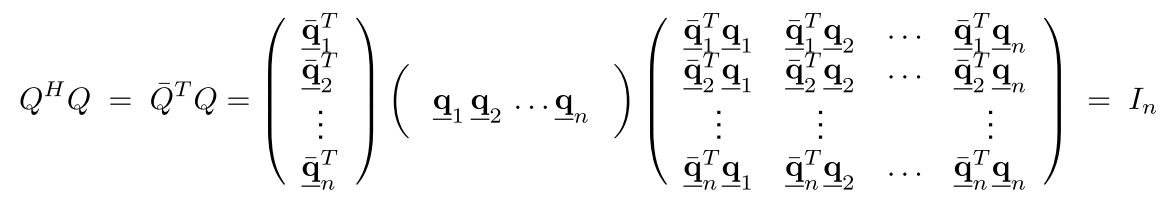
\includegraphics[scale=0.4]{1.JPG}
\end{figure}

\begin{tcolorbox}[breakable,colback=white]
\textbf{Unitary}: An invertible complex matrix satisfying $\bar{Q}^T Q = I_n$
\end{tcolorbox}

\pagebreak

An extremely useful unitary matrix is the DFT matrix, also called Fourier matrix.
\begin{figure} [h!]
    \centering
    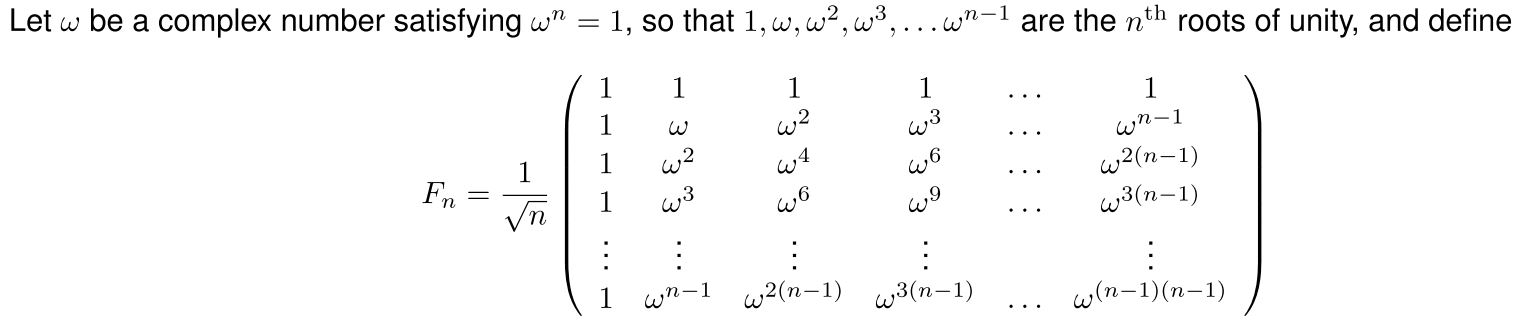
\includegraphics[scale=0.4]{2.JPG}
\end{figure}
\begin{figure} [h!]
    \centering
    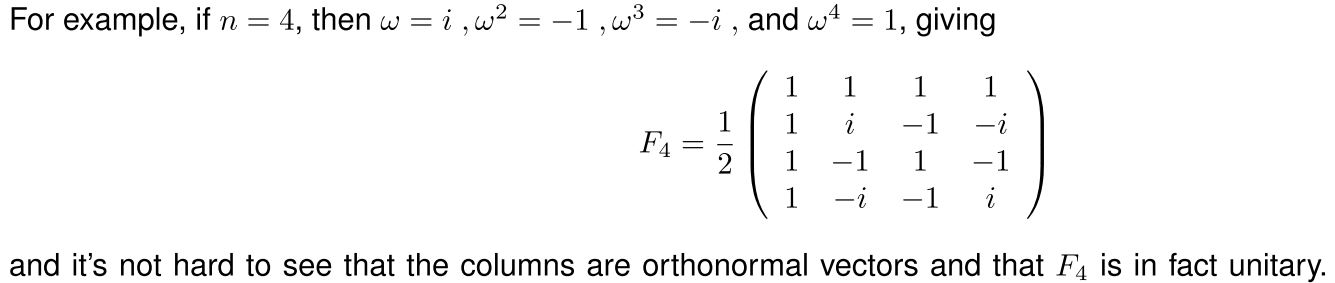
\includegraphics[scale=0.4]{3.JPG}
\end{figure}

%%%%%%%%%%%%%%%%%%%%%%%%%%%%%%%%%%%%%%%%%%%%%%%%%%%%%%%%%%%%%%%%%%%%%%%%%%%%%%%%%%%%%%%%%%%%%%%%%%%%%%%%%%
\subsection{Positive-definite Matrices}

\begin{tcolorbox}[breakable,colback=white]
\textbf{Positive-definite}: A symmetric matrix whose eigenvalues are all positive.
\end{tcolorbox}

A positive definite matrix needs to satisfy:
\begin{align*}
    \underline{\mathbf{x}}^{T}\left(A^{T} A\right) \underline{\mathbf{x}}>0 \quad \text { for every } \quad \underline{\mathbf{x}} \neq \underline{\mathbf{0}}
\end{align*}

%%%%%%%%%%%%%%%%%%%%%%%%%%%%%%%%%%%%%%%%%%%%%%%%%%%%%%%%%%%%%%%%%%%%%%%%%%%%%%%%%%%%%%%%%%%%%%%%%%%%%%%%%%
\subsection{The Singular Value Decomposition (SVD)}

The SVD is available for any matrix, including non-square unlike LU and QR.

Given any $m \times n$ matrix $A$, the Singular Value Decomposition of $A$ is
\begin{align*}
    A=U \Sigma V^{T}
\end{align*}

where $U$ and $V$ are orthogonal matrices (unitary, if complex numbers involved) and $\Sigma$ is
diagonal, though not necessarily square. $\Sigma$ will be $m \times n$ and will have zero-entries
everywhere except on the main diagonal, where $i = j$.

Note the sizes of each matrix:
\begin{figure} [h!]
    \centering
    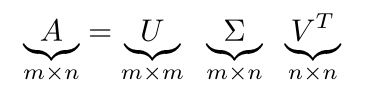
\includegraphics[scale=0.7]{4.JPG}
\end{figure}

\pagebreak

\textbf{Example 1}: Find the SVD of $A = \begin{pmatrix}
    2&2&0\\-1&1&0
\end{pmatrix}$

\begin{itemize}
    \item Note the rank: $r = 2$ - two \textbf{singular values} required
    \item Note the matrix size: $2\times 3$ matrix thus:
    \begin{itemize}
        \item $U = 2\times 2$
        \item $\Sigma = 2 \times 3$
        \item $V = 3 \times 3$
    \end{itemize}
    \item Find $A A^T$: 
    \begin{align*}
        A^T A = \begin{pmatrix}
            8&0\\0&2
        \end{pmatrix}
    \end{align*}
    \item Find the eigen values and vectors:
    \begin{itemize}
        \item Eigenvalues: $8$ and $2$
        \item Eigenvectors:
        \begin{align*}
            u_1 = \begin{pmatrix}
                1\\0
            \end{pmatrix}
            \; \text{ and } \;
            u_2 = \begin{pmatrix}
                0\\1
            \end{pmatrix}
        \end{align*}
    \end{itemize}
    \item List the singular values: $\sqrt{8}$ and $\sqrt{2}$
    \item Find the $V$ vector:
    
\end{itemize}


\pagebreak
%%%%%%%%%%%%%%%%%%%%%%%%%%%%%%%%%%%%%%%%%%%%%%%%%%%%%%%%%%%%%%%%%%%%%%%%%%%%%%%%%%%%%%%%%%%%%%%%%%%%%%%%%%
\subsection{Pseudoinverse}

If $A^{-1}$ does not exist for a given $A$, a pseudoinverse $A^+$ can be obtained by using the SVD.

\begin{align*}
    \underbrace{A^{+}}_{n \times m}=\underbrace{V}_{n \times n} \underbrace{\Sigma^{+}}_{n \times m} \underbrace{U^{T}}_{m \times m}=\left(\begin{array}{ccccccc}
        \frac{1}{\sigma_{1}} & 0 & 0 & \ldots & 0 & 0 & 0 \\
        0 & \frac{1}{\sigma_{2}} & 0 & \ldots & 0 & 0 & 0 \\
        \vdots & \vdots & \vdots & & \vdots & \vdots & \vdots \\
        0 & 0 & 0 & \ldots & \frac{1}{\sigma_{r}} & 0 & 0 \\
        0 & 0 & 0 & \ldots & 0 & 0 & 0 \\
        0 & 0 & 0 & \ldots & 0 & 0 & 0
        \end{array}\right)\left(\underline{\mathbf{u}}_{1} \underline{\mathbf{u}}_{2} \ldots \underline{\mathbf{u}}_{r} \underline{\mathbf{u}}_{r+1} \ldots \underline{\mathbf{u}}_{m}\right)^{T}
\end{align*}

When $A$ is invertible, then $A^+$ is the same as the inverse, but when not, we can still multiply
\begin{align*}
    A A^{+}=\left(U \Sigma V^{T}\right)\left(V \Sigma^{+} U^{T}\right)=U\left(\Sigma \Sigma^{+}\right) U^{T}
\end{align*}

where $\Sigma \Sigma ^+$ is an $m \times m$ diagonal matrix with $r$ ones on the diagonal and $m -
r$ zeroes. Multiplying by $U$ on the left and $U^T$ on the right leaves these in place and we end
up with
\begin{align*}
    A A^{+}=\Sigma \Sigma^{+}=\left(\begin{array}{cc}
        I_{r} & 0 \\
        0 & \underline{0}
        \end{array}\right)
\end{align*}

Note $AA^+$ and $A^+A$ are different:
\begin{align*}
    A^{+} A=\left(V \Sigma^{+} U^{T}\right)\left(U \Sigma V^{T}\right)=V \Sigma^{+} \Sigma V^{T}=\Sigma^{+} \Sigma=\left(\begin{array}{cc}
        I_{r} & 0 \\
        0 & \underline{0}
        \end{array}\right)
\end{align*}
The amount of zeroes on the diagonal in each case depends on $r$, $m$, $n$.

\begin{figure} [h!]
    \centering
    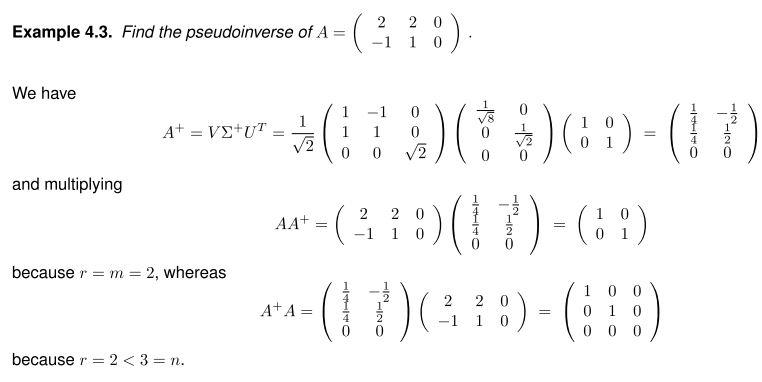
\includegraphics[scale=0.6]{5.JPG}
\end{figure}


%%%%%%%%%%%%%%%%%%%%%%%%%%%%%%%%%%%%%%%%%%%%%%%%%%%%%%%%%%%%%%%%%%%%%%%%%%%%%%%%%%%%%%%%%%%%%%%%%%%%%%%%%%
\end{document}